\chapter{Revisão bibliográfica}

No presente capítulo será discorrido a revisão bibliográfica do sistema de transmissão de energia sem fio apresentando o conceito, funcionamento, produtos disponíveis no mercado e, também, a teoria dos principais componentes utilizados no projeto.

\section{LASER}

Sinônimo de alta tecnologia e considerado uma das maiores invenções do século XX o \emph{Laser} (\emph{Light Amplification by Stimulated Emission of Radiation}) é um dispositivo que possibilita a amplificação da luz por emissão estimulada de radiação, essa característica o diferencia de fontes luminosas comuns proporcionando uma vasta gama de aplicações nas mais diversas áreas da indústria, medicina, militar, telecomunicações etc.

\subsection{Contexto histórico}

Em 1900, Max Planck, o ``Pai da Física Quântica'', descobriu que ``A radiação é absorvida ou emitida por um corpo aquecido através de pequenos `pacotes' de energia, mas não sob a forma de ondas''. Esses `pacotes', denominados quantum, são os fótons da energia eletromagnética que, segundo o físico dinamarquês Niels Bohr, também podem ser caracterizados como quantidade de energia absorvida ou emitida pelo elétron nas suas transições de órbitas.

A compreensão de que a luz é uma forma de partícula foi fundamental para o estudo de Einstein sobre emissão estimulada apresentado no ``The Quantum Theory of Radiation'' [6] que foi a primeira publicação sobre o conceito de radiação a laser.

A teoria de Albert Einstein diz que, um átomo perturbado por um fóton que incide sobre ele, emite um outro fóton de mesma fase, frequência, polarização e direção do original, esse processo ocorre como efeito cascata. A luz é gerada somente quando os fótons emitidos forem maiores do que os absolvidos.

Em uma época em que a exploração do espectro magnético era limitada, um grupo de cientistas norte-americanos e russos (Charles Townes, Jim Gordon, Nicolay Basov e Alexsander Prokhorov) desenvolveram separadamente, em 1954, um dispositivo que amplifica as micro-ondas, chamado de MASER (Microwave Amplification by Stimulated Emission of Radiation), ou seja, amplificação de micro-ondas pela emissão estimulada de radiação.

Utilizando amônia como meio ativo, o funcionamento deste dispositivo ocorre ao ser excitado por um agente externo, a molécula de amônia entra em vibração com uma frequência de micro-ondas e essa emissão estimulada gera um feixe coerente de micro-ondas. Essa descoberta é considerada o precursor do laser, o que lhes concedeu o prêmio Nobel de Física em 1964.

O primeiro laser foi apresentado em 16 de maio de 1960, pelo físico estadunidense Theodore Maiman, sendo o cristal de rubi o meio ativo do dispositivo.

\begin{quote}
Uma fonte de luz, na forma do poderoso clarão de uma lâmpada, irradiou um cristal de rubi sintético [com duas faces paralelas cobertas de prata], que absorveu energia sobre uma ampla banda de frequências. Essa energia ótica excitou os átomos até um estado de maior energia, do qual a energia foi irradiada novamente em uma estreita banda de frequências. Os átomos excitados foram acoplados a um ressonador óptico e estimulados a emitir juntos a radiação. (T. H. Maiman Nature 187, 493–494; 1960).
\end{quote}

Nas décadas seguintes, este instrumento passou a ser cada vez mais presente no cotidiano das pessoas e tornou-se fundamental nas mais diversas atividades, sendo utilizado em soldagens, impressoras, cirurgias, holografia, equipamentos de cirurgia dentária, leitores de CD e DVD, leitores de código de barra, ciência biomédica etc.

\subsection{Teoria}

Sabe-se que o fóton é emitido quando um átomo em um estado excitado ``cai'' para um estado de energia inferior, sendo que esse estado dura alguns nanosegundos. Átomos e moléculas podem também absorver fótons, efetuando então uma transição de um nível energético inferior para um superior. Quanto maior a temperatura, maior a probabilidade de ocorrer colisões, sendo que estas provocam transições para níveis energéticos superiores. [8]

Como foi mencionado no contexto histórico de Albert Einstein, baseando-se na mecânica quântica, teorizou o princípio do funcionamento do raio laser, no qual partia da emissão estimulada:

\begin{quote}
Se um átomo no estado excitado é iluminado por um fóton que tem a mesma energia da transição que ocorreria espontaneamente, o átomo pode ser estimulado a voltar ao estado de mais baixa energia e simultaneamente emitir um fóton com a mesma energia da transição e mesma direção do fóton incidente. Assim, um único fóton que interage com um átomo excitado pode resultar então em dois fótons. Se usarmos a descrição ondulatória da luz, a emissão estimulada terá a frequência da luz incidente e estará em fase (coerente), resultando em amplificação da intensidade da onda de luz original.[8]
\end{quote}

Segundo Zilio (2009, p.213) na ausência de colisões, as moléculas tendem a permanecer no estado energético mais baixo disponível. Ou seja, estados de energia alta são sempre menos povoados que o estado fundamental, sendo a absorção superior à emissão estimulada.

``A probabilidade da emissão estimulada é idêntica à probabilidade da absorção estimulada.'' (A. Einstein Phys. Z. 18, 121, 1917)

\begin{quote}
...como o número de átomos no estado excitado é muito pequeno com relação ao do estado fundamental, o fóton emitido tem uma probabilidade muito maior de ser re-absorvido, fazendo a emissão estimulada insignificante quando comparada com a emissão espontânea (no equilíbrio termodinâmico). O mecanismo pelo qual a emissão estimulada pode se tornar dominante é ter mais átomos no estado excitado que no estado fundamental, de forma que os fótons emitidos têm maior probabilidade de estimular a emissão do que serem absorvidos. Como esta condição é o inverso do que ocorre na situação de equilíbrio normal, ela é denominada de inversão de população. Havendo mais átomos num estado excitado que no fundamental, a emissão estimulada pode dominar, resultando numa cascata de fótons. O primeiro fóton emitido estimulará a emissão de mais fótons, que estimularão a emissão de ainda mais fótons, e assim por diante. A cascata resultante de fótons cresce, produzindo a amplificação da luz emitida. Se a inversão de população termina (a população do estado fundamental domina), a emissão espontânea se tornará novamente o processo favorecido.(Zilio, 2009, p.213)
\end{quote}

Para que a excitação do meio ativo ocorra é necessário utilizar uma fonte de excitação externa, ou seja, um mecanismo de bombeamento que varia conforme o meio escolhido, podendo ser lâmpadas flash, lâmpadas de arco, outro laser e etc.

No laser, a emissão de luz acontece somente quando o ganho supera as perdas, sendo que este ocorre quando há inversão de população, para que este fenômeno aconteça é necessário que os fótons fiquem confinados em uma cavidade ressonante, de forma a serem utilizados para desencadear mais processos de emissão estimulada, caso contrário, o sistema irradia para todas as direções.

A cavidade ressonante óptica é rodeada por dois espelhos, um parcialmente e o outro totalmente refletor, o que torna o processo de emissão estimulada maximizado, pois o feixe resultante é forçado a atravessar ciclicamente o meio ativo provocando o aumento da intensidade a cada volta completa (``round trip''). Além disso, esse processo faz com que a emissão ocorra em uma mesma fase, a propriedade de vibração em fase chama-se coerência espacial (RIBEIRO, 2000; SVELTO,2010).

Portanto, o dispositivo necessita satisfazer três condições fundamentais para operação:

\begin{itemize}
	\item Meio ativo: sólido, líquido ou gasoso;
	\item Mecanismo de excitação ou bombeamento;
	\item Ressonador ou cavidade ressonante.
\end{itemize}

As outras fontes luminosas são emitidas espontaneamente sem nenhuma intervenção externa apresentando ondas com diferentes comprimentos e frequência, de forma a viajar no espaço e tempo incoerentemente.

\subsection{Propriedades}

As suas características proporcionam propriedades diferenciadas em relação às outras demais fontes de luz. Assim, Bagnato (2001, p.9) aponta os principais aspectos:

\subsubsection{Monocromático}

A radiação ocorre em um único movimento de onda ou cor, portanto, possui um estreito intervalo de comprimento de onda. O brilho gera uma grande quantidade de luz, o feixe se propaga na mesma direção, havendo o mínimo de dispersão e a onda possui mesmo comprimento e fase. A tabela \ref{tab:comp_onda} mostra os comprimentos de onda para alguns tipos de laser.

\begin{table}[ht!]
	\caption{Principais comprimentos de onda}
	\label{tab:comp_onda}
	\begin{tabular}{c|c|c}
		\hline
		Laser & Cor & /lambda (nm)\\
		\hline
		\multirow{2}{*}{Ar} & Azul & 488\\
		\cline{2-3}
		& Verde & 514,5\\
		\hline
		\multirow{2}{*}{He-Ne} & Verde & 594,5\\
		\cline{2-3}
		& Vermelho & 632,8\\
		\hline
		\multirow{3}{*}{Kr} & Verde & 530,8\\
		\cline{2-3}
		& Amarelo & 568,2\\
		\cline{2-3}
		& Vermelho & 647,1\\
		\hline
		Rubi & Vermelho & 694,1\\
		\hline
		\multirow{3}{*}{GaAsAl} & Infravermelho & 790\\
		\cline{2-3}
		& Infravermelho & 830\\
		\cline{2-3}
		& Infravermelho & 904\\
		\hline
		Nd:YAG & Infravermelho & 1064\\
		\hline
		CO2 & Infravermelho & 10600\\
		\hline
	\end{tabular}
	\smallcaption{Fonte: Adaptado de \url{http://pelicano.ipen.br/PosG30/TextoCompleto/Martha\%20Simoes\%20Ribeiro_D.pdf}. Acessado em: 22/05/2021}
\end{table}

\subsubsection{Feixe Gaussiano}

Em condições ideais, a luz de um laser assume a forma de um Feixe Gaussiano, ou seja, a luz pode ser transportada e confinada na forma de feixe, apresentando mínima divergência. (SALEH; TEICH, 1991, p.81)

As principais características deste tipo de feixe óptico são:

\begin{itemize}
	\item A concentração de potência do feixe encontra-se dentro de um cilindro que envolve o eixo do feixe.
	\item A distribuição de intensidade em qualquer plano transversal é uma função gaussiana circularmente simétrica centrada em torno do feixe.
	\item A largura desta função é mínima na cintura do feixe e tornando-se gradualmente maior à medida que as distâncias entre entre as cintura aumentam nos dois sentidos.
	\item As frentes de ondas são aproximadamente planar perto da cintura do feixe, gradualmente se curva com o aumento da distância para a cintura, e em última instância, torna-se aproximadamente esférica longe da cintura.
	\item A divergência angular das normais de frente de onda assume o valor mínimo permitido pela equação de onda para uma determinada largura de feixe. Sob condições ideais, a partir de muitos tipos de laser, a luz toma a forma de um feixe de Gauss.
\end{itemize}

O modo gaussiano transversal fundamental (TEM) é o mais usado na maioria das aplicações lasers, sendo a amplitude complexa do feixe Gaussiano expressa em $U_{(r)}$ (SALEH; TEICH, 1991, p.83).

\begin{equation}
\label{eq:gaussiano}
U_{(r)}=A_0\frac{W_0}{W_{(z)}}exp\left [ -jkz-jk\frac{\rho ^2}{2R_{(z))}}+j\xi_{(z)} \right ]
\end{equation}

\begin{equation}
\label{eq:k_gaussiano}
k=2\frac{\pi}{\lambda}
\end{equation}

Onde $\rho$ é a distância radial ao eixo do feixe, $z$ distância axial a partir do foco do feixe, $k$ número de onda por comprimento de onda, $U$ amplitude do campo elétrico, $W$ raio do qual a amplitude tem decaimento de $1/e$, $W_{(0)}$ tamanho da cintura, $R$ raio de curvatura da frente de onda e $\xi$ é a fase de \emph{Gouy}.

O cálculo da equação \eqref{eq:gaussiano} determina as propriedades do feixe gaussiano [11]. Nas equações são considerados os parâmetros $A_0$ e $Z_0$ determinados pelas condições de fronteira e $\lambda$ que é o comprimento de onda.

\subsection{Largura de feixe}

Dentro de qualquer plano transversal, a intensidade do feixe, assume seu valor de pico no eixo e tem um fator de decaimento aproximadamente 0,135 na distância radial, $\rho$, conforme equação \eqref{eq:rho_gaussiano_largura}, sendo que 86\% da energia é transportada dentro de um círculo de raio $W_{(z)}$, considerando $W_{(z)}$ como o feixe do raio (também chamado de largura do feixe), equação (5). A largura RMS (\emph{Root Mean Squared}), $\sigma$, da distribuição de intensidade é dada pela equação \eqref{eq:sigma_gaussiano_largura}. [12]

\begin{equation}
\label{eq:rho_gaussiano_largura}
\rho = W_{(z)}
\end{equation}

\begin{equation}
\label{eq:sigma_gaussiano_largura}
\sigma = 1/2W_{(z)}
\end{equation}

\begin{equation}
\label{eq:gaussiano_largura}
W_{(z)} = W_0 \left [ 1 + \left( \frac{z}{z_0} \right ) ^2 \right ] ^{1/2}
\end{equation}

Assume-se valor mínimo $W_0$ no plano $z = 0$, denominado cintura do feixe. Assim $W_0$ é o raio da cintura. O diâmetro da cintura $2W_0$ é chamado de tamanho do ponto. (SALEH; TEICH, 1991, p.85)

\begin{equation}
\label{eq:raio_cintura_1}
W_0 = \left( \frac{\lambda z_0}{\pi} \right)^{1/2}
\end{equation}

\begin{equation}
\label{eq:raio_cintura_2}
W_{(z)} = \frac{\lambda z_0}{\pi} z = \theta_0 z
\end{equation}

\begin{figure}[ht!]
	\centering
	\caption{Optica do feixe}
	\label{fig:beam_optics}
	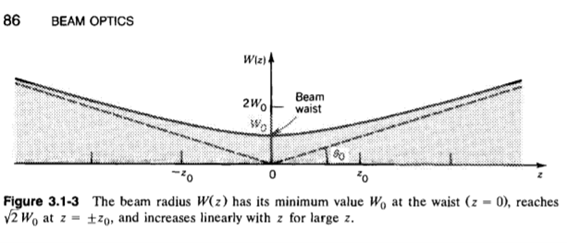
\includegraphics{beam_optics}[scale=1]
	\smallcaption{Fonte: SALEH, Bahaa E. A.; TEICH, Malvin Carl. Fundamentals of Photonics. 1.ed. Wiley-Interscience, 1991.}
	\smallcaption{Legenda: O raio do feixe $W_{(z)}$ tem seu valor mínimo no ponto eixo ($z = 0$), ele atinge $\sqrt{2} W_0$ quando $z=\pm z$, e aumenta linearmente com $z$ para valores de $z$ elevado.}
\end{figure}

\begin{equation}
\label{eq:raio_curvatura}
R_{(z)} = z \left [ 1 + \left( \frac{z}{z_0} \right ) ^2 \right ]
\end{equation}

\begin{equation}
\label{eq:fase_gouy}
\xi_{(z)} = tan^-1 \left( \frac{z}{z_0} \right )
\end{equation}

\begin{equation}
\label{eq:potencia_curvatura}
P=\frac{1}{2} I_0 \left( \pi W_0^2 \right )
\end{equation}

\begin{equation}
\label{eq:intensidade_eixo}
I_0 = \frac{E_0^2}{2 \eta}
\end{equation}

\begin{equation}
\label{eq:impedancia_meio}
\eta = \eta_0 \approx 377 \Omega
\end{equation}

Sendo o Raio de curvatura representado na equação \eqref{eq:raio_curvatura}, Fase de \emph{Gouy} representado na equação \eqref{eq:fase_gouy}, potência representado na equação \eqref{eq:potencia_curvatura} de acordo com e intensidade do eixo representado na equação \eqref{eq:intensidade_eixo}, sendo $\eta$ a impedância característica do meio, para o espaço livre (vide equação \eqref{eq:impedancia_meio}). Feixes ópticos são usualmente caracterizados pela potência $P$, então é útil escrever $I_0$ em temos de $P$ , equação \eqref{eq:i_p} [11].

\begin{equation}
\label{eq:i_p}
\eta = \eta_0 \approx 377 \Omega
\end{equation}

\subsubsection{Ângulo de divergência}

Longe do centro do feixe, o raio aumenta linearmente com $z$, definido um cone com meio ângulo \ang{80}, Figura \ref{fig:angulo_divergencia}, cerca de 86\% da potência do feixe é confinada dentro deste cone, sendo $\theta$ ângulo de divergência teta zero do feixe.

\begin{equation}
\label{eq:angulo_divergencia}
\theta_0 = \frac{2}{\pi} \frac{\lambda}{2 W_0}
\end{equation}

\begin{figure}[ht!]
	\centering
	\caption{Ângulo de divergência}
	\label{fig:angulo_divergencia}
	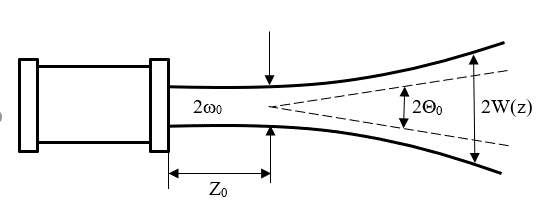
\includegraphics{angulo_divergencia}[scale=1]
	\smallcaption{Fonte: SALEH, Bahaa E. A.; TEICH, Malvin Carl. Fundamentals of Photonics. 1.ed. Wiley-Interscience, 1991.}
\end{figure}

\subsubsection{Profundidade de foco}

A profundidade de foco $Z_0$, é dada pela equação \ref{eq:prof_foco}, onde $\lambda$ é o comprimento de onda e $W_0$ é o raio do feixe na saída.

\begin{equation}
\label{eq:prof_foco}
2z_{0}=\frac{1 \pi W_0^2}{\lambda}
\end{equation}

\subsection{Segurança}

A colimação do feixe é o que difere a radiação do laser em relação aos outros tipos conhecidos de radiação, o comprimento de onda é o fator determinante para que o laser possa ser caracterizado como prejudicial. [12]

Na Figura \ref{espectro}, a parte amarela compreende o intervalo de comprimento de onda da atuação do laser.

\begin{figure}[ht!]
	\centering
	\caption{Intervalo do Espectro Eletromagnético onde o Laser atua}
	\label{fig:espectro}
	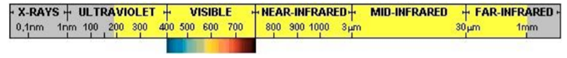
\includegraphics{espectro}[scale=1]
	\smallcaption{Fonte: Laser Institute of America, Laser Safety Information Bulletin, May 24, 2002.}
\end{figure}

Carroll [13] afirma que, em certas partes do corpo, tais como o globo ocular e os testículos, a conexão térmica com os tecidos circundantes é mínima e o fornecimento de sangue é inadequado para conduzir a energia desenvolvida pela exposição local ao laser. Quando estes órgãos estão expostos a tal tipo de radiação, podem produzir-se graves danos nos tecidos profundos dentro dos mesmos, onde há um grave risco de que causem cegueira ou esterilidade.

A periculosidade dos lasers infravermelhos se dá, principalmente, pelo fato da radiação invisível impossibilitar a resposta protetora de aversão ao brilho do corpo (``reflexo de piscar''), podendo causar danos imediatos na visão. Os demais efeitos biológicos da radiação podem ser consultados na Figura \ref{radiacao}.

\begin{figure}[ht!]
	\centering
	\caption{Efeitos biológicos da Radiação Laser}
	\label{fig:radiacao}
	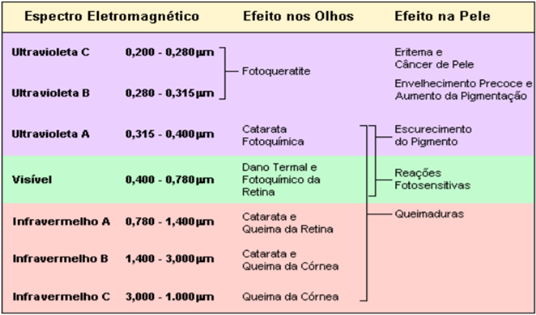
\includegraphics{radiacao}[scale=1]
	\smallcaption{Fonte: Laser Institute of America, Laser Safety Information Bulletin, May 24, 2002.}
\end{figure}

A maioria dos danos provocados pela radiação laser se deve ao aquecimento dos tecidos que a absorvem. Os lasers visíveis são particularmente perigosos, pois o olho humano focaliza o feixe na retina e esta pode sofrer queimaduras. A densidade de potência do ponto laser focalizado na retina é cerca de 100.000 vezes a densidade de potência incidente na córnea. Assim, embora seja relativamente seguro expor a pele a lasers visíveis de baixa potência, é sempre perigoso observar o feixe diretamente. [13]

Para realizar a avaliação dos riscos da exposição da radiação do laser, deve-se levar em conta as seguintes características:

\begin{itemize}
	\item Comprimento de onda;
	\item Potência;
	\item Duração e taxa de repetição;
	\item Diâmetro do feixe;
	\item Divergência.
\end{itemize}

\subsubsection{MPE}

A MPE (\emph{Maximum Permissible Exposure}) mede os níveis máximos permitidos de exposição levando em consideração a maior potência ou densidade de energia (\mbox{$W/cm^2$} ou \mbox{$J/cm^2$}) de uma fonte de luz que possa ser considerada segura. Essa medida é feita na córnea do olho humano ou pele, considerando o comprimento de onda, coerência temporal e coerência espacial. Na Tabela \ref{tab:mpe} pode-se observar o tempo máximo permitido de exposição em relação a alguns comprimentos de onda.

\begin{table}[ht!]
	\caption{Máxima exposição permitida}
	\label{tab:mpe}
	\begin{tabular}{c|c|c|c|c|c}
		\hline
		\multirow{2}{*}{\emph{Laser type}} & Wavelenght & MPE level (\mbox{$W/cm^2$})\\
		\cline{2-6}
		& (\mbox{$\mu$}) & 0.25 sec & 10 sec & 600 sec & 30,000 sec\\
		\hline
		
	\end{tabular}
	\smallcaption{Fonte: Adaptado de RIBEIRO, Martha Simões. INTERAÇÃO DA RADIAÇÃO LASER LINEARMENTE POLARIZADA DE BAIXA INTENSIDADE COM TECIDOS VIVOS: EFEITOS NA ACELERAÇÃO DE CICATRIZAÇÃO TISSULAR EM LESÕES DE PELE. 2000. 200 f. TCC}
\end{table}